%\chapter{Uma análise de domínio corporativo} - manter comentado

	\begin{flushright}
		\textit{``Não se possui o que não se compreende''.
		\\Johann Goethe}
	\end{flushright}


%Problema
%\textbf{Problema do capítulo: encontrar características do domínio corporativo.}
Este capítulo trata da caracterização do domínio corporativo e objetiva explicitar quais características da informação corporativa são comuns a diferentes instituições. Dessa forma, o capítulo apresenta uma proposta de generalização do domínio corporativo e ilustra algumas características descobertas a partir da análise de domínio utilizando as técnicas de análise de assunto e análise facetada, empreendidas em cada uma das coleções de documentos pesquisadas. Dentro do domínio corporativo, somente através de uma análise de domínio rigorosa pode-se tentar responder se as facetas adotadas por empresas diferentes apresentam alguma semelhança.


%Objetivo Geral
%O objetivo deste capítulo é determinar um conjunto mínimo de facetas para entidades corporativas que permita sua representação com um equilíbrio entre a expressividade de contexto e baixo custo computacional de reconhecimento e indexação de entidades corporativas por meio de métodos automáticos.

%São objetivos específicos a identificação das facetas que sejam comuns ao domínio corporativo; e também a identificação das características mais específicas que precisem ser estudadas e tratadas com atenção ao contexto e às necessidades de cada empresa, sob risco de não atender aos objetivos de recuperação de informação de seus respectivos usuários informacionais.

%Motivação/Justificativa

%Para o projeto de um sistema de recuperação de informação, muitas vezes é necessário ter contato com a coleção de documentos e necessidades de usuários. Para sistemas mais caros, é comum tentar generalizar seus usos dentro de um domínio para que o sistema seja distribuído com o menor custo. Do ponto de vista científico, a tentativa de generalização é uma curiosidade científica importante para garantir a evolução dos sistemas documentários, em geral, e de um domínio em particular.

%No entanto, toda e qualquer tentativa de generalização no domínio corporativo deve permanentemente enfrentar dificuldades de acesso a amostras de informação corporativa.




%Procedimento metodológico

%\textbf{Procedimentos metodológicos da análise de domínio.}
Os procedimentos metodológicos da análise de domínio foram executados como segue: i-a) análise de assuntos e o levantamento de termos mais significativos em cada uma das coleções de documentos; i-b) formação de assuntos pela leitura e pela aplicação das técnicas de dissecação e desnudação; ii) categorização dos assuntos pela aplicação da técnica da análise facetada em cada coleção de documentos; e iii) consolidação das categorias, facetas e subfacetas comuns às duas coleções de documentos.

%\textbf{Sumário para procedimentos metodológicos indicando suas respectivas seções e colocando os subprodutos nos anexos.}
Os procedimentos de análise, formação e categorização de assuntos (i-a, i-b e ii, respectivamente) foram executados em cada coleção, isoladamente, pelo autor deste trabalho. Os dois primeiros são reportados na seção \ref{analiseFormacaoDeAssuntos} e a categorização é reportada na seção \ref{categorizacao}. Todos os assuntos devidamente categorizados estão disponíveis nos anexos \ref{anexoassuntosCEFETMGdocs}, \ref{anexoassuntosCSIROqueries} e \ref{anexoassuntosCSIROdocs}.

%\textbf{Sumário para o produto preliminar da análise de domínio corporativo.}
Por último, a análise preliminar do domínio corporativo é encerrada pelo procedimento de consolidação das facetas comuns às coleções e de avaliação do grau de similaridade que tais facetas supostamente apresentam no domínio. Seus resultados são apresentados e discutidos na seção \ref{analiseDominioRes}.


\section{Análise de assuntos e formação de assuntos}
\label{analiseFormacaoDeAssuntos}

%\textbf{Propósito da análise de assuntos.}\footnote{Inverti os parágrafos, como pediu.}
A análise de assuntos constitui a análise intelectual dos documentos de cada coleção com o propósito de interpretá-los e de representar seus assuntos por meio de termos em linguagem natural. Em seguida, sobre os assuntos resultantes foram aplicadas as técnicas de dissecação e desnudação para formação de assuntos adicionais. O processamento da análise e formação de assuntos foi dividido em três fases e ocorreu linearmente sobre as coleções particular e pública, nessa ordem.

%\textbf{Análise de assuntos sobre as duas coleções.}\footnote{Você pediu para eu colocar algo como ``Primeiramente foi analisada a coleção particular seguindo as propostas: leitura..., análise dos documentos, seleção dos termos representativos, ...''. Porém, observe que essas operações já estão no segundo parágrafo deste capítulo. Por que coloquei assim? Porque são 3 amostras de 2 coleções. Os mesmos procedimentos metodológicos de análise são aplicados nas 3 amostras. Logo, ao invés de repetir antes de cada amostra, eu falo uma vez só no início do capítulo. Ok? Eu melhorei a descrição dos procedimentos, adicionando mais detalhes da formação de assuntos, como pediu.}
A análise de assuntos foi realizada sobre duas coleções de documentos provenientes de duas empresas, o Centro Federal de Educação Tecnológica de Minas Gerais (CEFETMG) e a \textit{Commonwealth Scientific and Industrial Research Organisation} (CSIRO). Como as coleções pertencem a empresas diferentes, sua comparação dá-se pelos assuntos corporativos que ambas tratam. Isto é, dois assuntos, mesmo representados por termos distintos, podem ser considerados idênticos por uma avaliação intelectual do classificador. É o caso do assunto país, representado igualmente por Brasil ou \textit{Australia}; de instituição, representado por CEFETMG ou CSIRO; e de serviço, representado por Curso de graduação ou por \textit{Research}. Por outro lado, um mesmo termo pode referir-se a assuntos diferentes para cada empresa. Um exemplo é o termo \textit{site} que denota um \textit{Web site} ou um local de funcionamento da empresa para a CSIRO, enquanto só representa o primeiro assunto para a empresa CEFETMG. 


\subsection{Primeira fase de processamento: documentos da coleção particular}

%\textbf{Explicação sobre a coleção particular.}
A primeira fase de processamento da análise de assuntos ocorreu sobre a coleção particular de documentos que pertencem à empresa CEFETMG. A coleção particular foi produzida por um gerente da empresa como um conjunto significativo e útil de documentos para o trabalho rotineiro e para tomada de decisão. Esses documentos estavam organizados em repositórios, sendo possível encontrar réplicas de um documento em um ou mais repositórios. Os repositórios mobilizados constituem a principal fonte de informação que gerentes e usuários de informação têm usado na empresa entre os anos de 2012 e 2013; portanto essa coleção é mais eficaz que uma amostra aleatória do arquivo corrente para o propósito desta pesquisa. A tabela \ref{tab:documentosParticular} apresenta os repositórios a que pertencem os documentos com a quantidade de documentos e páginas oriundos de cada um.

% Booktabs require to add \usepackage{booktabs} to your document preamble
\begin{table}[h]
\caption{Composição da coleção particular}
\centering
\begin{tabular}{@{}lrrr@{}}
\toprule
                               & \multicolumn{1}{c}{\textbf{Documentos (D)}} & \multicolumn{1}{c}{\textbf{Páginas (P)}} & \multicolumn{1}{c}{\textbf{P/D}} \\ \midrule
Formulários                    & 9                                           & 11                                       & 1,2                              \\ %\midrule
Atas de Informática            & 11                                          & 28                                       & 2,5                              \\ %\midrule
Páginas Web                    & 5                                           & 5                                        & 1                                \\ %\midrule
Atas da Congregação            & 55                                          & 124                                      & 2,3                              \\ %\midrule
Atas do Fórum de Coordenadores & 14                                          & 45                                       & 3,2                              \\ %\midrule
Notícias externas              & 210                                         & 210                                      & 1                                \\ %\midrule
Notícias internas              & 384                                         & 384                                      & 1                                \\ %\midrule
Projetos                       & 4                                           & 426                                      & 106,5                            \\ %\midrule
Normas internas                & 6                                           & 107                                      & 17,8                             \\ %\midrule
Normas externas                & 1                                           & 109                                      & 109                              \\ %\midrule
Correspondências               & 606                                         & 606                                      & 1                                \\ \midrule
\textbf{Total}                 & \textbf{1305}                               & \textbf{2055}                            & \textbf{1,6}                     \\ \bottomrule
\end{tabular}
\label{tab:documentosParticular}
\legend{Fonte: Elaborada pelo autor.}
\end{table}

%Validação? Amostral? Kappa?

%\textbf{Levantamento dos assuntos.}
Um único profissional da área, autor desta tese, leu 1305 documentos produzidos entre os anos de 2007 e 2013 e anotou os assuntos presentes na medida em que foram identificados. Nessa etapa, os assuntos foram anotados através do termo em linguagem natural que melhor o representava, empregando a terminologia adotada pela instituição em pelo menos um documento da coleção. O documento onde o assunto/termo aparecia pela primeira vez também foi anotado, mas esse dado não é disponibilizado nesta tese por violar o acordo de sigilo. O objetivo é evitar constrangimentos por provável informação, e.g.: o termo Joseph ocorre pela primeira vez em um processo disciplinar.

\begin{figure}
	\caption{\label{fig:assuntosIdentificadosParticular}Novos assuntos descobertos em repositórios da coleção particular}

	\centering
		\includegraphics[width=1.0\textwidth]{fig/assuntosIdentificadosParticular.jpg}

	\legend{Fonte: elaborada pelo autor}
\end{figure}

%\textbf{Dissecação e desnudação aplicadas.}
Após a leitura de cada documento e a anotação dos novos assuntos descobertos, foram aplicados os métodos de dissecação e desnudação para formação de assuntos adicionais. 

Através do método de dissecação se divide o universo analisado em lâminas, sendo que cada lâmina representa um assunto básico ou um isolado. Por meio de um processo iterativo, as lâminas são dividas em novas lâminas de níveis diferentes. Um exemplo de formação de assuntos pela aplicação do método de dissecação é o renque Manhã, Noite e Tarde para turnos de trabalho. 

Através do método de desnudação são identificados assuntos com grande profundidade a partir de assuntos mais gerais ou isolados. O resultado é uma cadeia de assuntos em que a profundidade aumenta e a extensão diminui a cada iteração do método.
Um exemplo de formação de assuntos pelo método de desnudação, é a cadeia Ensino $\supset$ Ensino médio e profissional técnico de nível médio $\supset$ Ensino técnico.
Ou seja, Ensino técnico é subconjunto de Ensino médio e profissional técnico de nível médio, que está contido em Ensino.

Os demais três métodos de formação de assuntos, laminação, agregação e sobreposição, não foram utilizados na amostra, uma vez que foi usada a linguagem natural presente na amostra, inexistindo vocabulário controlado para controle terminológico.

%\textbf{Assuntos resultantes.}
A figura \ref{fig:assuntosIdentificadosParticular} mostra a ordem de processamento, do repositório de formulários ao repositório de Emails, e o número de novos assuntos descobertos em cada repositório da coleção particular. Porém, caso outra ordem de processamento fosse seguida o total de assuntos descobertos continuaria o mesmo. A análise e formação de assuntos na coleção particular consumiu o tempo total de 29 horas e 20 minutos e resultou em 1643 assuntos que estão listados no anexo \ref{anexoassuntosCEFETMGdocs}. 



\subsection{Segunda fase de processamento: queries e narrativas da coleção pública}

%\textbf{Explicação sobre a coleção pública.}
A segunda fase de processamento da análise de assuntos ocorreu sobre a coleção de referência pública usada na trilha \textit{Enterprise} da \textit{Text Retrieval Conference} (TREC) até o ano de 2008. Trata-se de uma coleção de 370715 páginas \textit{Web} públicas da empresa CSIRO; além de um conjunto de 77 narrativas e 77 \textit{queries} disponibilizadas por funcionários da CSIRO como as questões mais frequentemente respondidas por funcionários da CSIRO para clientes externos \cite{bailey07csiro}. Apenas as narrativas e \textit{queries} foram adotadas nesta segunda fase. As narrativas correspondem a uma questão de exemplo escrita por um cliente e enviada para funcionários da CSIRO. Para responder a questão do cliente, um funcionário deve realizar uma ou mais buscas no sistema de recuperação de informação da empresa. Essa busca é constituída por um exemplo de \textit{query} que retorna documentos pertinentes para responder a questão.

%\textbf{Explicação sobre as narrativas e queries que fazem parte da coleção pública.}
As narrativas e as \textit{queries} apresentam termos e assuntos que podem ser vistos como índices para 19650 documentos classificados como ``altamente relevantes'' para as necessidades de busca de seus clientes e funcionários, o que corresponde 5,3\% de toda a coleção composta por 370715 documentos. Dessa forma, as narrativas e as queries foram usadas partindo do pressuposto de que elas são suficientes como índice para os termos e assuntos mais frequentes para clientes e especialistas de informação da empresa.

%\textbf{Levantamento dos assuntos.}
O mesmo profissional da primeira fase leu as 77 narrativas e \textit{queries} em pares enquanto anotava os assuntos presentes. Nessa etapa, os assuntos foram anotados através do termo em linguagem natural que melhor o representava pelo emprego da terminologia adotada pelo cliente (no caso das narrativas), pela instituição (no caso das \textit{queries}) ou por ambos.

%\textbf{Dissecação e desnudação aplicadas.}
Após a leitura de cada par narrativa-\textit{query} e a anotação dos novos assuntos descobertos, foram aplicadas as técnicas de dissecação e desnudação para formação de assuntos adicionais. 

%Através do método de dissecação se divide o universo analisado em lâminas, sendo que cada lâmina representa um assunto básico ou um isolado. Por meio de um processo iterativo, as lâminas são dividas em novas lâminas de níveis diferentes. 
Tendo em vista que as narrativas e \textit{queries}, as quais compõem a amostra da segunda fase, apresentam um escopo mais limitado, nenhum assunto foi produzido por dissecação. Através do método de desnudação, pelo qual se produz cadeias de assuntos em que a profundidade aumenta e a extensão diminui a cada iteração do método, houve formação de assuntos.
Um exemplo de formação de assuntos pelo método de desnudação nessa fase é a cadeia \textit{Australia} $\supset$ \textit{New South Wales} $\supset$ Sydney para a hierarquia espacial da cidade de Sydney.
Ou seja, \textit{Sydney} está contida em \textit{New South Wales}, que está contida em \textit{Australia}.

Os demais três métodos de formação de assuntos, laminação, agregação e sobreposição, não foram utilizados na amostra, uma vez que foi usada a linguagem natural presente na amostra, inexistindo vocabulário controlado para controle terminológico.

%\textbf{Assuntos resultantes.}
Os assuntos descobertos na primeira e segunda fases de processamento foram categorizados e as duas coleções sofreram uma primeira comparação antes que a terceira fase de processamento acontecesse. Os procedimentos e o resultado da categorização encontra-se na seção \ref{categorizacao}; os procedimentos e o resultado da comparação entre as coleções encontra-se na seção \ref{analiseDominioRes}; porém, a execução dos procedimentos e obtenção dos resultados da terceira fase, descritos na próxima seção \ref{terceira}, caso realizados imediatamente após as duas primeiras fases, não alterariam a comparação entre coleções. A análise e formação de assuntos de narrativas e \textit{queries} da coleção pública consumiu o tempo total de 42 horas e 11 minutos e resultou em 241 assuntos que estão listados no anexo \ref{anexoassuntosCSIROqueries}. 


%A análise de assunto através da leitura de tantas páginas Web é inviável para os limite de tempo que esta pesquisa possui. Por outro lado, a leitura da totalidade do repositório apresentaria resultados diferentes, o que não significa resultados mais úteis ou precisos. A análise de assunto então ocorreu exclusivamente sobre o que a comunidade científica julgou relevante e a comunidade profissional da CSIRO julgou útil.

%Ao fazer dessa forma, a principal desvantagem é limitar em excesso a terminologia adotada pelo CSIRO e eventualmente adotar uma terminologia do cliente que não é usada internamente na empresa. Por outro lado, foi reduzido o esforço de leitura intelectual e foi esse trabalho teve a primeira possibilidade de comparação direta dos resultados dos participantes da TREC e os resultados obtidos neste trabalho.

%A classificação de relevância e pertinência dos resultados é tomada como correta e adequada, mesmo pressuposto dos trabalhos encontrados na literatura. Um profissional de informação externo à CSIRO dificilmente conseguiria fazer um melhor julgamento que o profissional que se encontrava inserido em seu contexto corporativo ou que tenha realizado a indexação coletivamente durante a TREC.

%Os resultados empíricos alcançados pela comunidade científica não foram validados pelos profissionais de informação da CSIRO. Por isso devem ser usados com cautela.

%As 77 consultas e 77 narrativas desempenham o papel de representação dos documentos que servem como validação para a avaliação empírica do nosso modelo.

%Porém, ambas utilizam-se de linguagem natural em texto corrente, sendo que mereceram uma reescrita onde apenas as palavras mais significativas foram preservadas.

%Isso precisa de validação?

%A totalidade dos assuntos resultantes é apresentada no anexo \ref{assuntosCSIROqueries}, com uma classificação em três níveis que explica o significado do termo em linguagem natural, no contexto da empresa estudada.



%Using the private and public collections, the subject and facet analyses were done by reading all the documents from the private collection (see Table 1); 77 queries and 77 narratives of user needs from the public collection; and 50 documents from the public collection.


%No entanto, a adoção das duas coleções possui duas funções: validar a coleção pública como uma coleção corporativa; e validar a coleção particular como uma coleção de teste.

\subsection{Terceira fase de processamento: documentos da coleção pública}
\label{terceira}

%\textbf{Explicação sobre a coleção pública usada na terceira fase.}
Na terceira fase de processamento foi feita a análise de assuntos sobre a coleção de referência pública usada na trilha \textit{Enterprise} da \textit{Text Retrieval Conference} (TREC) até o ano de 2008. Porém, nesta fase o interesse eram os documentos da coleção e não mais as narrativas e \textit{queries}. Como a coleção é constituída por 370715 páginas \textit{Web} públicas e sua leitura demandaria mais tempo que aquele possível para a pesquisa, uma amostra de apenas 50 documentos foi analisada intelectualmente.

%\textbf{Explicação sobre a amostra de documentos que faz parte da coleção pública.}
Para constituir a amostra, foram selecionados os 19650 documentos considerados altamente relevantes para as 77 narrativas e \textit{queries} processadas na segunda fase de processamento. Os documentos foram ordenados pela quantidade de narrativas e \textit{queries} em que eram considerados altamente relevantes. Os 50 documentos mais frequentes em narrativas e \textit{queries} (0,254\% do total de documentos altamente relevantes) foram então selecionados para a terceira fase, sendo comuns a um mínimo de 25 narrativas e \textit{queries}. Em média, os 50 documentos estão associados a 36,46 narrativas e \textit{queries} com desvio padrão de 6,8756.

%\textbf{Levantamento dos assuntos.}
O mesmo profissional das duas primeiras fases leu os 50 documentos enquanto anotava os assuntos presentes. Nesta fase, os assuntos foram anotados através do termo em linguagem natural que melhor o representava pelo emprego da terminologia adotada pela instituição. Após a leitura de cada documento e a anotação dos novos assuntos descobertos, foram aplicadas as técnicas de dissecação e desnudação para formação de assuntos adicionais. 

Através do método de dissecação são produzidos renques dentro de facetas. Um exemplo de formação de assuntos pela aplicação da técnica de dissecação é o renque New South Wales (NSW), Queensland (Qld), South Australia (SA), Tasmania (Tas), Victoria (Vic) e Western Australia (WA) de estados australianos.

Através do método de desnudação são identificados assuntos com grande profundidade a partir de assuntos mais gerais ou isolados.% O resultado é uma cadeia de assuntos em que a profundidade aumenta e a extensão diminui a cada iteração do método.
Um exemplo de formação de assuntos pelo método de desnudação, é a cadeia não exaustiva \textit{Energy Technology} $\supset$ \textit{Energy Centre} $\supset$ \textit{National Solar Energy Centre}, de unidades organizacionais da divisão de pesquisa da CSIRO em tecnologia energética.
Ou seja, \textit{National Solar Energy Centre} está contida na unidade \textit{Energy Centre}, que está contida na diretoria de \textit{Energy Technology}.

Os demais três métodos de formação de assuntos, laminação, agregação e sobreposição, não foram utilizados na amostra, uma vez que foi usada a linguagem natural presente na amostra, inexistindo vocabulário controlado para controle terminológico.

%\textbf{Assuntos resultantes.}
Os assuntos descobertos foram categorizados e as facetas resultantes foram comparadas com aquelas das duas fases anteriores, como é visto nas seções \ref{categorizacao} e \ref{analiseDominioRes} respectivamente. A terceira fase de análise e formação de assuntos na coleção pública consumiu um tempo adicional de 27 horas e 51 minutos e resultou em 913 assuntos que estão listados no anexo \ref{anexoassuntosCSIROdocs}.



\section{Categorização de assuntos através da análise facetada}
\label{categorizacao}

%\textbf{Explicação sobre a estrutura classificatória com 3 níveis.}
Após o processamento de cada uma das três fases descritas na seção anterior, os assuntos reconhecidos pelo processo de análise foram categorizados em uma estrutura classificatória com três níveis. O primeiro nível representa as categorias fundamentais, o segundo nível representa as facetas pelas quais cada categoria é dividida, enquanto o terceiro nível constitui as subfacetas pelas quais cada faceta é dividida.

Categorias, facetas e subfacetas emergiram da análise facetada pela necessidade de categorizar os assuntos reconhecidos nas amostras. Isto é, a estrutura não foi definida arbitrariamente antes de o processo de categorização ocorrer. Os nomes das categorias, facetas e subfacetas não servem para atribuir significado. Por outro lado, o significado de cada uma delas pode ser deduzido facilmente pela posição em que cada uma ocupa na estrutura classificatória facetada.

As categorias, facetas e subfacetas consolidadas a partir das três amostras são:




\begin{multicols}{2}
\begin{itemize}	\item Categoria \textbf{Associação} -- onde residem os assuntos relacionados às instituições associadas a instituição proprietária da coleção -- dividida em	\begin{enumerate} 	\item Aquisição	\begin{enumerate} 	\item Nome de empresa	\end{enumerate}	
			\item Atendimento	\begin{enumerate} 	\item Nome de recurso	\end{enumerate}	
			\item Cliente	\begin{enumerate} 	\item Nome de unidade	\end{enumerate}	
			\item Comunicação	\begin{enumerate} 	\item Nome de veículo		
					\item Tipo de veículo	\end{enumerate}	
			\item Concorrência	\begin{enumerate} 	\item Apelido de empresa		
					\item Nome de empresa		
					\item Nome de serviço	\end{enumerate}	
			\item Financiador	\begin{enumerate} 	\item Nome de empresa	\end{enumerate}	
			\item Fornecedor	\begin{enumerate}			
					\item Nome de empresa		
					\item Nome de serviço		
			\item Fusão			\end{enumerate}	
			\item Grupo	\begin{enumerate} 	\item Nome de empresa	\end{enumerate}	
			\item Influência	\begin{enumerate} 	\item Apelido de pessoa		
					\item Nome de empresa		
					\item Nome de pessoa		
					\item Nome de unidade		
					\item Papel de pessoa		
					\item Poder público	\end{enumerate}	
			\item Parceria	\begin{enumerate}			
					\item Apelido de empresa		
					\item Modalidade		
					\item Nome de empresa		
					\item Nome de pessoa		
					\item Site de empresa		
					\item Tipo de parceiro	\end{enumerate}	
			\item Parte	\begin{enumerate}			
					\item Função		
					\item Nome de empresa		
			\item Profissional			\end{enumerate}	
			\item Sindicato	\begin{enumerate}			
					\item Nome de empresa	\end{enumerate}	
\end{enumerate}	\item Categoria \textbf{Comunicação} -- onde residem os assuntos relacionados aos canais de comunicação mobilizados na instituição -- dividida em	\begin{enumerate} 	\item Correspondência				
			\item Email				
			\item Internet				
			\item Rádio				
			\item Telefone				
			\item Televisão				
\end{enumerate}	\item Categoria \textbf{Conhecimento} -- onde residem os assuntos relacionados às áreas de conhecimento e profissionais -- dividida em	\begin{enumerate} 	\item Área				
\end{enumerate}	\item Categoria \textbf{Documento} -- onde residem os assuntos relacionados aos documentos, seu ciclo de vida, suas características físicas e metadados -- dividida em	\begin{enumerate} 	\item Acervo	\begin{enumerate}			
					\item Banco de dados		
					\item e-book		
					\item Livro		
					\item Material	\end{enumerate}	
			\item Anais				
			\item Artigo				
			\item Assunto				
			\item Atualização				
			\item Autorização				
			\item Avaliação				
			\item Blog				
			\item Coleção				
			\item Conjunto				
			\item Contrato	\begin{enumerate}			
					\item Alteração	\end{enumerate}	
			\item Entrega	\begin{enumerate}			
					\item Data		
					\item Meio	\end{enumerate}	
			\item Fluxo				
			\item Folheto				
			\item Formato de documento				
			\item Formulário				
			\item Gênero de documento	\begin{enumerate}	\item Ata		
					\item Carta		
					\item Certificado		
					\item Declaração		
					\item Edital		
					\item Extrato		
					\item Fluxograma		
					\item Laudo		
					\item Notícia		
					\item Parecer		
					\item Planilha		
					\item Portaria		
					\item Projeto		
					\item Questionário		
					\item Resolução	\end{enumerate}	
			\item Identificação				
			\item Idioma				
			\item Imagem				
			\item Legislação				
			\item Lista				
			\item Livreto				
			\item Livro				
			\item Manual				
			\item Mapa				
			\item Marca				
			\item Modelo				
			\item Norma				
			\item Palavra-chave				
			\item Parte				
			\item Podcast				
			\item Portifólio				
			\item Preservação				
			\item Produção				
			\item Regulamento				
			\item Relatório				
			\item Réplica				
			\item Requerimento	\begin{enumerate}			
					\item Assunto		
					\item Situação	\end{enumerate}	
			\item Roteiro				
			\item Site	\begin{enumerate}			
					\item Endereço	\end{enumerate}	
			\item Suporte				
			\item Tamanho				
			\item Versão				
			\item Vídeo				
\end{enumerate}	\item Categoria \textbf{Economia} -- onde residem assuntos relacionados às características das atividades econômicas e da moeda -- dividida em	\begin{enumerate} 	\item Arranjo produtivo				
			\item Atividade econômica	\begin{enumerate}			
					\item Educação	\end{enumerate}	
			\item Moeda				
			\item Porte				
\end{enumerate}	\item Categoria \textbf{Espaço} -- onde residem assuntos georreferenciáveis -- dividida em	\begin{enumerate} 	\item Cidade	\begin{enumerate}			
					\item Apelido de cidade		
					\item Bairro		
					\item Endereço		
					\item Equipamento urbano		
					\item Logradouro		
					\item Região		
					\item Região urbana	\end{enumerate}	
			\item Continente				
			\item Distrito federal				
			\item Estado	\begin{enumerate}			
					\item Região estadual	\end{enumerate}	
			\item Medida				
			\item País	\begin{enumerate}			
					\item Região		
					\item Rodovia	\end{enumerate}	
			\item Região	\begin{enumerate}			
					\item Bloco econômico	\end{enumerate}	
\end{enumerate}	\item Categoria \textbf{Instituição} -- onde residem assuntos relacionados à empresa e às unidades organizacionais da empresa -- dividida em	\begin{enumerate} 	\item Apelido de empresa				
			\item Atualização				
			\item Cultura				
			\item Nome de empresa				
			\item Tipo de instituição				
			\item Unidade	\begin{enumerate}			
					\item Papel	\end{enumerate}	
			\item Visão				
\end{enumerate}	\item Categoria \textbf{Operação} -- onde residem assuntos relacionados às atividades de produção e de gerenciamento dos processos organizacionais da empresa -- dividida em 	\begin{enumerate} 	\item Atendimento	\begin{enumerate}			
					\item Área de atendimento		
					\item Capacidade		
					\item Desempenho		
					\item Equipe		
					\item Expansão		
					\item Frequência		
					\item Interrupção		
					\item Método		
					\item Nome de evento		
					\item Pós-venda		
					\item Produto		
					\item Projeto		
					\item Tipo de evento	\end{enumerate}	
			\item Cobrança				
			\item Compra	\begin{enumerate}			
					\item Pagamento	\end{enumerate}	
			\item Controle	\begin{enumerate}			
					\item Alocação		
					\item Análise		
					\item Apresentação		
					\item Avaliação externa		
					\item Decisão		
					\item Desempenho		
					\item Discussão		
					\item Equipe		
					\item Frequência		
					\item Pendência		
					\item Reunião		
					\item Sanção		
					\item Seleção	\end{enumerate}	
			\item Desenvolvimento	\begin{enumerate}			
					\item Avaliação		
					\item Equipe		
					\item Papel		
					\item Produto		
					\item Projeto	\end{enumerate}	
			\item Divulgação	\begin{enumerate}			
					\item Instrumento		
					\item Meio		
					\item Nome de evento		
					\item Público-alvo		
					\item Tipo de evento		
					\item Venda	\end{enumerate}	
			\item Estoque				
			\item Financiamento	\begin{enumerate}			
					\item Captação		
					\item Modalidade		
					\item Seleção		
			\item Informática		\item Nome de sistema	\end{enumerate}	
			\item Manutenção	\begin{enumerate}			
					\item Equipe	\end{enumerate}	
			\item Orçamento	\begin{enumerate}			
					\item Alocação	\end{enumerate}	
			\item Pessoal	\begin{enumerate}			
					\item Admissão		
					\item Alocação		
					\item Avaliação		
					\item Capacitação		
					\item Competência		
					\item Demissão		
					\item Equipe		
					\item Inventário		
					\item Licença		
					\item Nome de evento		
					\item Plano de saúde		
					\item Progressão		
					\item Remuneração		
					\item Seleção		
					\item Transferência		
					\item Vaga	\end{enumerate}	
			\item Produto				
			\item Segurança				
			\item Situação				
			\item Suporte à operação	\begin{enumerate}			
					\item Apelido de recurso		
					\item Infraestrutura		
					\item Nome de recurso	\end{enumerate}	
			\item Transporte	\begin{enumerate}			
					\item Equipamento		
					\item Evidência	\end{enumerate}	
			\item Venda	\begin{enumerate}			
					\item Produto	\end{enumerate}	
\end{enumerate}	\item Categoria \textbf{Patrimônio} -- onde residem assuntos relacionados aos bens móveis e imóveis -- dividida em	\begin{enumerate} 	\item Atualização				
			\item Depreciação				
			\item Equipamento				
			\item Imóvel	\begin{enumerate}			
					\item Construção		
					\item Equipamento		
					\item Infraestrutura		
					\item Projeto	\end{enumerate}	
			\item Licença de software				
			\item Participação societária				
\end{enumerate}	\item Categoria \textbf{Pessoal} -- onde residem assuntos relacionados às pessoas naturais, internas e externas à instituição -- dividida em	\begin{enumerate} 	\item Cliente	\begin{enumerate}			
					\item Conjunto		
					\item Idade		
					\item Papel		
					\item Responsável		
					\item Situação		
					\item Tempo de vínculo	\end{enumerate}	
			\item Comunidade				
			\item Desenvolvimento				
			\item Externo	\begin{enumerate}			
					\item Apelido		
					\item Nome		
					\item Papel		
					\item Profissão		
					\item Situação	\end{enumerate}	
			\item Filiação				
			\item Fornecedor	\begin{enumerate}	\item Prestador de serviço	\end{enumerate}	
			\item Grupo	\begin{enumerate}			
					\item Papel	\end{enumerate}	
			\item Identificação				
			\item Profissional	\begin{enumerate}			
					\item Competência		
					\item Conjunto		
					\item Email		
					\item Equipe		
					\item Formação		
					\item Função		
					\item Lotação		
					\item Modalidade		
					\item Modalidade de contratação		
					\item Nome		
					\item Origem		
					\item Papel		
					\item Profissão		
					\item Remuneração		
					\item Sobrenome		
					\item Status		
					\item Tempo de vínculo		
					\item Título acadêmico	\end{enumerate}	
			\item Sexo				
\end{enumerate}	\item Categoria \textbf{Procedimento} -- onde residem assuntos relacionados a tarefas desenvolvidas internamente na instituição -- não dividida em facetas						
	\item Categoria \textbf{Tempo} -- onde residem assuntos de referência temporal -- dividida em	\begin{enumerate} 	\item Alocação				
			\item Ano				
			\item Ano especial				
			\item Atualização				
			\item Calendário				
			\item Cronograma				
			\item Data				
			\item Década				
			\item Evento	\begin{enumerate}			
					\item Tipo de evento	\end{enumerate}	
			\item Fuso horário				
			\item Hora				
			\item Hora especial				
			\item Horário				
			\item Mês				
			\item Período	\begin{enumerate}			
					\item Intervalo		
					\item Intervalo em anos		
					\item Intervalo em dias		
					\item Intervalo em horas		
					\item Intervalo em meses	\end{enumerate}	
			\item Projeção				
			\item Século				
			\item Semana				
			\item Valor				
\end{enumerate} \end{itemize}
\end{multicols}





\begin{comment}

%\scriptsize
\begin{center}
%\begin{longtable}{p{4cm}|l|l|l|l}
\begin{longtable}{l|l|l}
\caption[Categorias, facetas e subfacetas consolidadas]{Categorias, facetas e subfacetas consolidadas}
\label{catfatsub}

\hline \textbf{Categoria} & \textbf{Faceta} & \textbf{Subfaceta} \\ \hline 
\endfirsthead

\multicolumn{3}{c}%
{{\bfseries \tablename\ \thetable{} -- continuação da página anterior}} \\
\hline \textbf{Categoria} & \textbf{Faceta} & \textbf{Subfaceta} \\ \hline 
\endhead

\hline \multicolumn{3}{r}{{Continua na próxima página}} \\ \hline
\endfoot

%\hline % Retirada para incluir Fonte.
\endlastfoot



Associação	&	Aquisição	&	Nome de empresa	\\ 	\hline
	&	Atendimento	&	Nome de recurso	\\ 	\hline
	&	Cliente	&	Nome de unidade	\\ 	\hline
	&	Comunicação	&	Nome de veículo	\\ 	
	&		&	Tipo de veículo	\\ 	\hline
	&	Concorrência	&	Apelido de empresa	\\ 	
	&		&	Nome de empresa	\\ 	
	&		&	Nome de serviço	\\ 	\hline
	&	Financiador	&	Nome de empresa	\\ 	\hline
	&	Fornecedor	&	--	\\ 	
	&		&	Nome de empresa	\\ 	
	&		&	Nome de serviço	\\ 	\hline
	&	Fusão	&	--	\\ 	\hline
	&	Grupo	&	Nome de empresa	\\ 	\hline
	&	Influência	&	Apelido de pessoa	\\ 	
	&		&	Nome de empresa	\\ 	
	&		&	Nome de pessoa	\\ 	
	&		&	Nome de unidade	\\ 	
	&		&	Papel de pessoa	\\ 	
	&		&	Poder público	\\ 	\hline
	&	Parceria	&	--	\\ 	
	&		&	Apelido de empresa	\\ 	
	&		&	Modalidade	\\ 	
	&		&	Nome de empresa	\\ 	
	&		&	Nome de pessoa	\\ 	
	&		&	Site de empresa	\\ 	
	&		&	Tipo de parceiro	\\ 	\hline
	&	Parte	&	--	\\ 	
	&		&	Função	\\ 	
	&		&	Nome de empresa	\\ 	\hline
	&	Profissional	&	Nome de empresa	\\ 	\hline
	&	Sindicato	&	--	\\ 	
	&		&	Nome de empresa	\\ 	\hline
Comunicação	&	Correspondência	&	--	\\ 	\hline
	&	Email	&	--	\\ 	\hline
	&	Internet	&	--	\\ 	\hline
	&	Rádio	&	--	\\ 	\hline
	&	Telefone	&	--	\\ 	\hline
	&	Televisão	&	--	\\ 	\hline
Conhecimento	&	Área	&	--	\\ 	\hline
Documento	&	Acervo	&	--	\\ 	
	&		&	Banco de dados	\\ 	
	&		&	e-book	\\ 	
	&		&	Livro	\\ 	
	&		&	Material	\\ 	\hline
	&	Anais	&	--	\\ 	\hline
	&	Artigo	&	--	\\ 	\hline
	&	Assunto	&	--	\\ 	\hline
	&	Atualização	&	--	\\ 	\hline
	&	Autorização	&	--	\\ 	\hline
	&	Avaliação	&	--	\\ 	\hline
	&	Blog	&	--	\\ 	\hline
	&	Coleção	&	--	\\ 	\hline
	&	Conjunto	&	--	\\ 	\hline
	&	Contrato	&	--	\\ 	
	&		&	Alteração	\\ 	\hline
	&	Entrega	&	--	\\ 	
	&		&	Data	\\ 	
	&		&	Meio	\\ 	\hline
	&	Fluxo	&	--	\\ 	\hline
	&	Folheto	&	--	\\ 	\hline
	&	Formato de documento	&	--	\\ 	\hline
	&	Formulário	&	--	\\ 	\hline
	&	Gênero de documento	&	Ata	\\ 	
	&		&	Carta	\\ 	
	&		&	Certificado	\\ 	
	&		&	Declaração	\\ 	
	&		&	Edital	\\ 	
	&		&	Extrato	\\ 	
	&		&	Fluxograma	\\ 	
	&		&	Laudo	\\ 	
	&		&	Notícia	\\ 	
	&		&	Parecer	\\ 	
	&		&	Planilha	\\ 	
	&		&	Portaria	\\ 	
	&		&	Projeto	\\ 	
	&		&	Questionário	\\ 	
	&		&	Resolução	\\ 	\hline
	&	Identificação	&	--	\\ 	\hline
	&	Idioma	&	--	\\ 	\hline
	&	Imagem	&	--	\\ 	\hline
	&	Legislação	&	--	\\ 	\hline
	&	Lista	&	--	\\ 	\hline
	&	Livreto	&	--	\\ 	\hline
	&	Livro	&	--	\\ 	\hline
	&	Manual	&	--	\\ 	\hline
	&	Mapa	&	--	\\ 	\hline
	&	Marca	&	--	\\ 	\hline
	&	Modelo	&	--	\\ 	\hline
	&	Norma	&	--	\\ 	\hline
	&	Palavra-chave	&	--	\\ 	\hline
	&	Parte	&	--	\\ 	\hline
	&	Podcast	&	--	\\ 	\hline
	&	Portifólio	&	--	\\ 	\hline
	&	Preservação	&	--	\\ 	\hline
	&	Produção	&	--	\\ 	\hline
	&	Regulamento	&	--	\\ 	\hline
	&	Relatório	&	--	\\ 	\hline
	&	Réplica	&	--	\\ 	\hline
	&	Requerimento	&	--	\\ 	
	&		&	Assunto	\\ 	
	&		&	Situação	\\ 	\hline
	&	Roteiro	&	--	\\ 	\hline
	&	Site	&	--	\\ 	
	&		&	Endereço	\\ 	\hline
	&	Suporte	&	--	\\ 	\hline
	&	Tamanho	&	--	\\ 	\hline
	&	Versão	&	--	\\ 	\hline
	&	Vídeo	&	--	\\ 	\hline
Economia	&	Arranjo produtivo	&	--	\\ 	\hline
	&	Atividade econômica	&	--	\\ 	
	&		&	Educação	\\ 	\hline
	&	Moeda	&	--	\\ 	\hline
	&	Porte	&	--	\\ 	\hline
Espaço	&	Cidade	&	--	\\ 	
	&		&	Apelido de cidade	\\ 	
	&		&	Bairro	\\ 	
	&		&	Endereço	\\ 	
	&		&	Equipamento urbano	\\ 	
	&		&	Logradouro	\\ 	
	&		&	Região	\\ 	
	&		&	Região urbana	\\ 	\hline
	&	Continente	&	--	\\ 	\hline
	&	Distrito federal	&	--	\\ 	\hline
	&	Estado	&	--	\\ 	
	&		&	Região estadual	\\ 	\hline
	&	Medida	&	--	\\ 	\hline
	&	País	&	--	\\ 	
	&		&	Região	\\ 	
	&		&	Rodovia	\\ 	\hline
	&	Região	&	--	\\ 	
	&		&	Bloco econômico	\\ 	\hline
Instituição	&	Apelido de empresa	&	--	\\ 	\hline
	&	Atualização	&	--	\\ 	\hline
	&	Cultura	&	--	\\ 	\hline
	&	Nome de empresa	&	--	\\ 	\hline
	&	Tipo de instituição	&	--	\\ 	\hline
	&	Unidade	&	--	\\ 	
	&		&	Papel	\\ 	\hline
	&	Visão	&	--	\\ 	\hline
Operação	&	Atendimento	&	--	\\ 	
	&		&	Área de atendimento	\\ 	
	&		&	Capacidade	\\ 	
	&		&	Desempenho	\\ 	
	&		&	Equipe	\\ 	
	&		&	Expansão	\\ 	
	&		&	Frequência	\\ 	
	&		&	Interrupção	\\ 	
	&		&	Método	\\ 	
	&		&	Nome de evento	\\ 	
	&		&	Pós-venda	\\ 	
	&		&	Produto	\\ 	
	&		&	Projeto	\\ 	
	&		&	Tipo de evento	\\ 	\hline
	&	Cobrança	&	--	\\ 	\hline
	&	Compra	&	--	\\ 	
	&		&	Pagamento	\\ 	\hline
	&	Controle	&	--	\\ 	
	&		&	Alocação	\\ 	
	&		&	Análise	\\ 	
	&		&	Apresentação	\\ 	
	&		&	Avaliação externa	\\ 	
	&		&	Decisão	\\ 	
	&		&	Desempenho	\\ 	
	&		&	Discussão	\\ 	
	&		&	Equipe	\\ 	
	&		&	Frequência	\\ 	
	&		&	Pendência	\\ 	
	&		&	Reunião	\\ 	
	&		&	Sanção	\\ 	
	&		&	Seleção	\\ 	\hline
	&	Desenvolvimento	&	--	\\ 	
	&		&	Avaliação	\\ 	
	&		&	Equipe	\\ 	
	&		&	Papel	\\ 	
	&		&	Produto	\\ 	
	&		&	Projeto	\\ 	\hline
	&	Divulgação	&	--	\\ 	
	&		&	Instrumento	\\ 	
	&		&	Meio	\\ 	
	&		&	Nome de evento	\\ 	
	&		&	Público-alvo	\\ 	
	&		&	Tipo de evento	\\ 	
	&		&	Venda	\\ 	\hline
	&	Estoque	&	--	\\ 	\hline
	&	Financiamento	&	--	\\ 	
	&		&	Captação	\\ 	
	&		&	Modalidade	\\ 	
	&		&	Seleção	\\ 	\hline
	&	Informática	&	Nome de sistema	\\ 	\hline
	&	Manutenção	&	--	\\ 	
	&		&	Equipe	\\ 	\hline
	&	Orçamento	&	--	\\ 	
	&		&	Alocação	\\ 	\hline
	&	Pessoal	&	--	\\ 	
	&		&	Admissão	\\ 	
	&		&	Alocação	\\ 	
	&		&	Avaliação	\\ 	
	&		&	Capacitação	\\ 	
	&		&	Competência	\\ 	
	&		&	Demissão	\\ 	
	&		&	Equipe	\\ 	
	&		&	Inventário	\\ 	
	&		&	Licença	\\ 	
	&		&	Nome de evento	\\ 	
	&		&	Plano de saúde	\\ 	
	&		&	Progressão	\\ 	
	&		&	Remuneração	\\ 	
	&		&	Seleção	\\ 	
	&		&	Transferência	\\ 	
	&		&	Vaga	\\ 	\hline
	&	Produto	&	--	\\ 	\hline
	&	Segurança	&	--	\\ 	\hline
	&	Situação	&	--	\\ 	\hline
	&	Suporte à operação	&	--	\\ 	
	&		&	Apelido de recurso	\\ 	
	&		&	Infraestrutura	\\ 	
	&		&	Nome de recurso	\\ 	\hline
	&	Transporte	&	--	\\ 	
	&		&	Equipamento	\\ 	
	&		&	Evidência	\\ 	\hline
	&	Venda	&	--	\\ 	
	&		&	Produto	\\ 	\hline
Patrimônio	&	Atualização	&	--	\\ 	\hline
	&	Depreciação	&	--	\\ 	\hline
	&	Equipamento	&	--	\\ 	\hline
	&	Imóvel	&	--	\\ 	
	&		&	Construção	\\ 	
	&		&	Equipamento	\\ 	
	&		&	Infraestrutura	\\ 	
	&		&	Projeto	\\ 	\hline
	&	Licença de software	&	--	\\ 	\hline
	&	Participação societária	&	--	\\ 	\hline
Pessoal	&	Cliente	&	--	\\ 	
	&		&	Conjunto	\\ 	
	&		&	Idade	\\ 	
	&		&	Papel	\\ 	
	&		&	Responsável	\\ 	
	&		&	Situação	\\ 	
	&		&	Tempo de vínculo	\\ 	\hline
	&	Comunidade	&	--	\\ 	\hline
	&	Desenvolvimento	&	--	\\ 	\hline
	&	Externo	&	--	\\ 	
	&		&	Apelido	\\ 	
	&		&	Nome	\\ 	
	&		&	Papel	\\ 	
	&		&	Profissão	\\ 	
	&		&	Situação	\\ 	\hline
	&	Filiação	&	--	\\ 	\hline
	&	Fornecedor	&	Prestador de serviço	\\ 	\hline
	&	Grupo	&	--	\\ 	
	&		&	Papel	\\ 	\hline
	&	Identificação	&	--	\\ 	\hline
	&	Profissional	&	--	\\ 	
	&		&	Competência	\\ 	
	&		&	Conjunto	\\ 	
	&		&	Email	\\ 	
	&		&	Equipe	\\ 	
	&		&	Formação	\\ 	
	&		&	Função	\\ 	
	&		&	Lotação	\\ 	
	&		&	Modalidade	\\ 	
	&		&	Modalidade de contratação	\\ 	
	&		&	Nome	\\ 	
	&		&	Origem	\\ 	
	&		&	Papel	\\ 	
	&		&	Profissão	\\ 	
	&		&	Remuneração	\\ 	
	&		&	Sobrenome	\\ 	
	&		&	Status	\\ 	
	&		&	Tempo de vínculo	\\ 	
	&		&	Título acadêmico	\\ 	\hline
	&	Sexo	&	--	\\ 	\hline
Procedimento	&	--	&	--	\\ 	\hline
Tempo	&	Alocação	&	--	\\ 	\hline
	&	Ano	&	--	\\ 	\hline
	&	Ano especial	&	--	\\ 	\hline
	&	Atualização	&	--	\\ 	\hline
	&	Calendário	&	--	\\ 	\hline
	&	Cronograma	&	--	\\ 	\hline
	&	Data	&	--	\\ 	\hline
	&	Década	&	--	\\ 	\hline
	&	Evento	&	--	\\ 	
	&		&	Tipo de evento	\\ 	\hline
	&	Fuso horário	&	--	\\ 	\hline
	&	Hora	&	--	\\ 	\hline
	&	Hora especial	&	--	\\ 	\hline
	&	Horário	&	--	\\ 	\hline
	&	Mês	&	--	\\ 	\hline
	&	Período	&	--	\\ 	
	&		&	Intervalo	\\ 	
	&		&	Intervalo em anos	\\ 	
	&		&	Intervalo em dias	\\ 	
	&		&	Intervalo em horas	\\ 	
	&		&	Intervalo em meses	\\ 	\hline
	&	Projeção	&	--	\\ 	\hline
	&	Século	&	--	\\ 	\hline
	&	Semana	&	--	\\ 	\hline
	&	Valor	&	--	\\ 	
\hline\hline						





\hline
\hline \multicolumn{3}{l}{Fonte: Elaborada pelo autor.}

\end{longtable}
\end{center}
%\normalsize

\end{comment}

%\textbf{Aplicação do processo de categorização da análise facetada.}
Então, os assuntos passaram pelo processo de categorização da análise facetada e as categorias encontradas podem ser vistas como um meio de comparação entre as coleções públicas e privadas. A análise facetada ocorreu sobre cada um dos assuntos identificados em cada fase do processamento de assuntos, com conferência e correções ao longo do processo. Após concluir a análise facetada sobre os três conjuntos de assuntos, uma nova iteração de correções e ajustes ocorreu com o objetivo de garantir consistência à categorização, entre os assuntos e as coleções.

%\textbf{Processo de síntese não ocorreu.}
O processo de síntese da técnica de análise facetada, quando assuntos compostos são formados pela combinação de conceitos, não foi implementado nesta tese. Isso se justifica pela importância de se reconhecer assuntos e termos relevantes para autores e usuários de cada coleção, ao invés de se tentar enumerar as quase infinitas possibilidades de assuntos que podem ocorrer nas coleções.

%\textbf{Princípios da AF que foram usados.}
%\footnote{Este parágrafo é novo, porque você tem algo parecido na sua tese! Li na sua tese e vi que citou os princípios no capítulo. Porém, na minha tese, prefiro mantê-los nas seções citadas no parágrafo e lembrar ao leitor os princípios que foram usados e aqueles que não foram usados. Caso o leitor precise de explicações fundamentais, ele precisa ir até a seção correspondente a cada plano (das ideias, verbal ou notacional).}
A formação das categorias respeitou os nove princípios do plano das ideias compilados por \citeonline{spiteri98simplified} e discutidos na seção \ref{planoDasIdeias}. O reconhecimento e a atribuição de significado à terminologia respeitou os dois princípios do plano verbal compilados por \citeonline{spiteri98simplified} e ainda respeitou o cânone da reticência de \citeonline{ranganathan1967}, explicados e discutidos na seção \ref{planoVerbal}. Os princípios do plano notacional não foram considerados nesta tese, uma vez que não foi produzido um sistema notacional para o sistema de classificação. Em outras palavras, a principal linguagem de trabalho usada pelo profissional da área e pelo usuário da informação foi a própria linguagem natural presente nos documentos.

%\textbf{Exemplos de categorização de assuntos.}
Um exemplo de resultado da categorização é o termo ``bluetongue disease'', categorizado como Operação-Desenvolvimento-Produto. Outros termos foram categorizados através de dois níveis da estrutura de classificação. É o caso do termo ``new south wales'', categorizado como Espaço-Estado. Também há termos categorizados através de apenas um nível, tal como o termo ``identification'' categorizado como Procedimento. Adicionalmente, um termo pode ser categorizado diferentemente entre as coleções e documentos, uma vez que a atenção é voltada para o significado e para a categoria do significado associados com o termo. No entanto, o método de análise facetada tentou ajustar sua atenção para todo o domínio constituído por ambas as coleções ao invés de restringir-se apenas ao escopo de um único e isolado documento, de apenas uma das coleções. Em outras palavras, a análise facetada não foi usada para categorizar documentos ou termos, mas para representar os assuntos emergidos dos documentos através de termos da linguagem natural.

%\textbf{Link para a próxima seção.}
Ao final, a avaliação da estrutura classificatória de três níveis ocorreu sobre o resultado consolidado das duas coleções. As categorias, facetas e subfacetas resultantes são analisadas na próxima seção \ref{analiseDominioRes}.


\section{Avaliação de categorias, facetas e subfacetas}
\label{analiseDominioRes}

%\textbf{Explicação sobre a comparação dos resultados e sumário para as próximas seções.}
A avaliação da estrutura classificatória e a comparação entre as duas coleções deram-se em cada um dos níveis da classificação, sendo que o primeiro nível está associado às categorias fundamentais, o segundo nível está associado às suas facetas e o terceiro nível está associado às subfacetas. Os três níveis são tratados nas subseções \ref{avaliacao-categorias}, \ref{avaliacao-facetas} e \ref{avaliacao-subfacetas}, respectivamente.

\subsection{Categorias}
\label{avaliacao-categorias}

%\textbf{12 categorias encontradas.}
Doze categorias emergiram da análise facetada e agrupam os assuntos resultantes dos documentos da coleção particular, das narrativas e \textit{queries} da coleção pública e dos documentos da coleção pública. As categorias são Pessoal, Associação, Instituição, Documento, Comunicação, Economia, Conhecimento, Operação, Procedimento, Espaço, Patrimônio e Tempo. A figura \ref{fig:facetasDocsQueries} ilustra a frequência com a qual assuntos foram categorizados em cada uma das categorias do primeiro nível da estrutura classificatória, onde a coleção pública ainda encontra-se dividida entre as narrativas e \textit{queries} (\textit{queries} da CSIRO) e os documentos (documentos da CSIRO).

%\textbf{3 categorias mais frequentes.}
Em ordem decrescente, as categorias Operação, Documento e Pessoal são as categorias com mais assuntos em qualquer das coleções. Isso indica que o conteúdo corporativo frequentemente apresenta características próprias para diferentes etapas da sua atividade econômica, para diferentes gêneros de documento e para diferentes indivíduos que atuam na empresa. Em outras palavras, é possível afirmar que o conteúdo corporativo orbita em torno das suas operações; se manifesta em gêneros textuais e de documentos, que apesar de poucos são explicitados por sua função de dar forma ao conteúdo; e são produzidos por e endereçados a indivíduos, ou ainda podem usar da autoridade de indivíduos para ter aumentada sua difusão. No entanto, a categoria Operação isoladamente agrupa entre 30\% e 50\%  de todos os assuntos que ocorrem nas coleções, as categorias Documento e Pessoal, isoladamente, agrupam um máximo de 15\% de todos os assuntos que ocorrem em cada coleção e as demais categorias em média agrupam 10\% de todos os assuntos.

%\textbf{Explicação da figura e do reagrupamento das categorias em 6.}
A figura \ref{fig:facetasDocsQueries} também agrupa as 12 categorias resultantes pela sua natureza tal como Entidades sociais, Mensagens, Disciplinas científicas, Processos de negócios, Espaço e Tempo. Por essa estrutura, o grupo de Processos de negócios, onde se encontra a categoria Operação, é aquele com o maior número de assuntos, mesmo sem o suporte da categoria Procedimentos. Entidades sociais, o segundo maior grupo, agrupa as categorias Pessoal (humanos), Instituição (pessoas jurídicas) e Associação (relações entre humanos, pessoas jurídicas e ambos). Em seguida, Mensagens posiciona-se como terceiro maior grupo principalmente por agrupar os assuntos da categoria Documentos, mas equipara-se ao grupo de Espaço. Espaço agrupa duas categorias, Espaço e Patrimônio, sendo que a primeira está ligada a nomes geográficos comuns ao ambiente corporativo e a segunda está ligada a equipamentos corporativos que podem ser georreferenciados. O quarto maior grupo é o Tempo, constituído por uma categoria com o mesmo nome, o que reflete a importância do tempo para as mensagens corporativas, dando a elas contexto temporal e validade limitada. Finalmente, Disciplinas científicas agrupa as categorias de Economia (atividades econômicas, principalmente) e Conhecimento (profissões e campos de estudo, principalmente). O último grupo demonstra o quanto esses assuntos são escassos nas mensagens corporativas, possivelmente porque as profissões e áreas de conhecimento sejam conhecidas \textit{a priori} pelos receptores das mensagens corporativas e portanto não precisam ser marcadas explicitamente no conteúdo das mensagens.

%\textbf{Explicação dos 6 agrupamentos.}
Os seis agrupamentos de categorias são muito semelhantes às cinco categorias fundamentais de Ranganathan, sendo o grupo Entidades sociais compatível com a categoria Personalidade; os grupos Mensagens e Disciplinas científicas compatíveis com a categoria Matéria; o grupo Processos de negócios compatível com a categoria Energia; e os grupos Espaço e Tempo compatíveis com as categorias fundamentais de mesmo nome. Associando-os dessa forma, a categoria fundamental energia constitui aquela com maior frequência nas coleções investigadas (com cerca de 50\% dos assuntos existentes), enquanto as outras categorias fundamentais apresentam igual frequência (com cerca de 10\% dos assuntos existentes, cada uma). 

%\textbf{Demonstração da correlação entre as coleções via figuras.}
As observações sobre categorias e grupos de categorias são comuns às duas coleções. As figuras \ref{fig:disp-docdoc} e \ref{fig:disp-docquery} demonstram graficamente a correlação entre o resultado da categorização entre documentos da coleção particular e pública, e entre o resultado da categorização entre documentos da coleção particular e narrativas e \textit{queries} da coleção pública. %Usando o coeficiente de correlação de Spearman, observamos uma alta correlação positiva com um $\rho = 0,9338, n = 2, p < 0,002$.

%\textbf{Demonstração da correlação entre coleção e query da CSIRO.}
Adicionalmente, pela figura \ref{fig:disp-docqueryCSIRO} pode ser observado que tanto as mensagens corporativas quanto as buscas construídas por profissionais de informação, passando pelas mensagens de clientes, apresentam a mesma distribuição de assuntos e facetas. Isto é, em uma busca, os usuários informacionais tendem a incluir assuntos associados às facetas identificadas com alta correlação positiva se comparados aos assuntos presentes nos documentos de interesse. A figura \ref{fig:disp-docqueryCSIRO} compara documentos da coleção pública com narrativas e \textit{queries} da coleção pública, enquanto a figura \ref{fig:disp-docquery} compara documentos da coleção particular com narrativas e \textit{queries} da coleção pública.





\begin{figure}
	\caption{\label{fig:facetasDocsQueries}Frequência de assuntos em cada categoria}

	\centering
		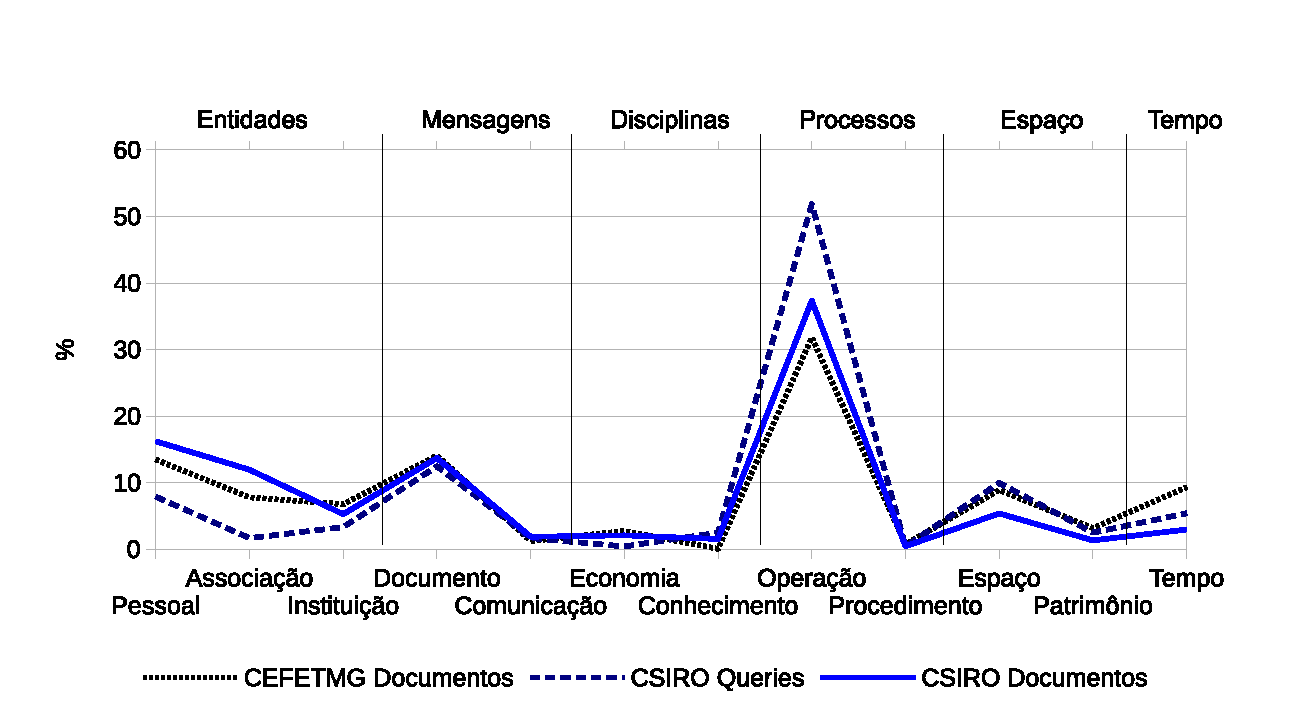
\includegraphics[width=1.0\textwidth]{fig/subjects-pt-docsqueries.eps}

	\legend{Fonte: elaborada pelo autor}
\end{figure}







\begin{figure}
	\caption{\label{fig:disp-docdoc}Dispersão da categorização de assuntos presentes em documentos do CEFETMG e da CSIRO}

	\centering
		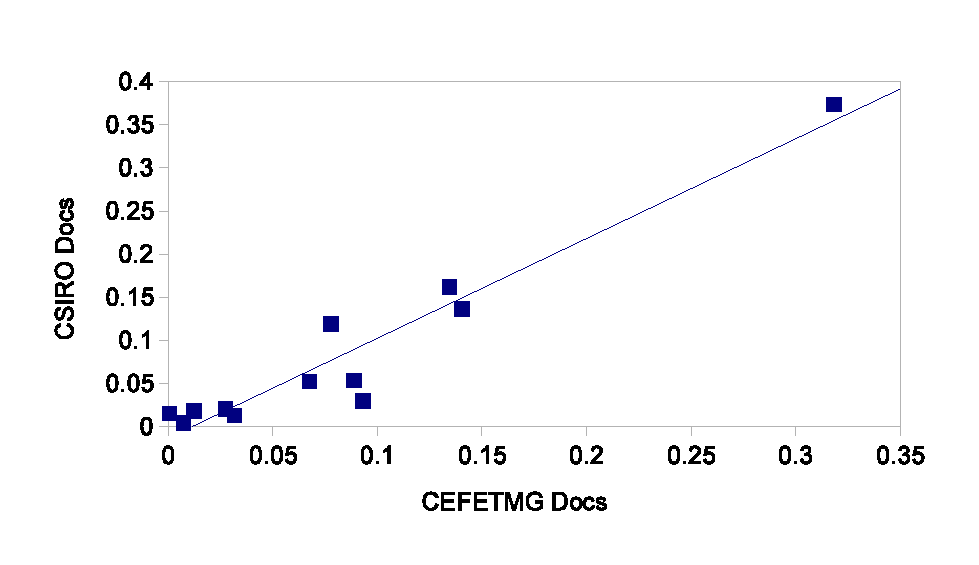
\includegraphics[width=1.0\textwidth]{fig/disp-docdoc.eps}

	\legend{Fonte: elaborada pelo autor}
\end{figure}







\begin{figure}
	\caption{\label{fig:disp-docqueryCSIRO}Dispersão da categorização de assuntos presentes em documentos da CSIRO e em queries da CSIRO}

	\centering
		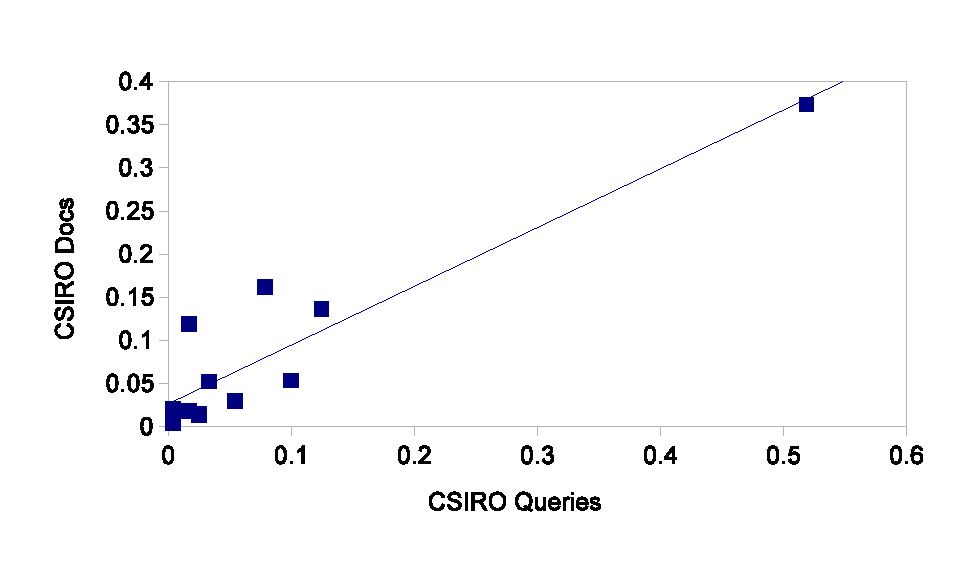
\includegraphics[width=1.0\textwidth]{fig/disp-docqueryCSIRO.eps}

	\legend{Fonte: elaborada pelo autor}
\end{figure}







\begin{figure}
	\caption{\label{fig:disp-docquery}Dispersão da categorização de assuntos presentes em documentos do CEFETMG e em queries da CSIRO}

	\centering
		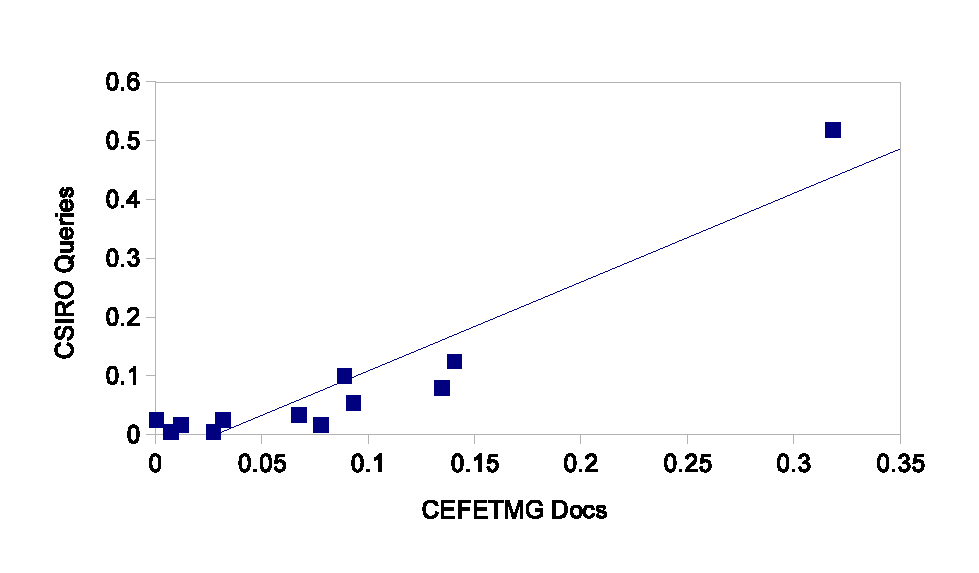
\includegraphics[width=1.0\textwidth]{fig/disp-docquery.eps}

	\legend{Fonte: elaborada pelo autor}
\end{figure}


%\textbf{Link para a próxima seção.}
Apesar de as coleções apresentarem semelhanças no nível mais alto da estrutura classificatória, as diferenças surgem e aumentam na medida em que níveis mais precisos de classificação são mobilizados. A próxima seção \ref{avaliacao-facetas} avança um nível na hierarquia da classificação e trata das facetas pelas quais cada categoria foi dividida.



\subsection{Facetas de categorias}
\label{avaliacao-facetas}

%\textbf{148 facetas resultantes.}
Ao avançar para o segundo nível da estrutura de classificação, as 12 categorias fundamentais são divididas em 148 facetas diferentes. Entre os assuntos da coleção particular, do conjunto de narrativas e \textit{queries}, e da amostra documentos da coleção pública, 97,56\%, 95,02\% e 98,13\% dos assuntos são classificados pelo menos até o nível de facetas.

%\textbf{Facetas da categoria 1.}
Em ordem alfabética, Associação é a primeira categoria, dividida em 14 facetas. Dentre elas, a faceta Parceria é a mais frequente e reúne assuntos relacionados a entidades que tenham relação de cooperação com a empresa original. Outras facetas populares em ordem alfabética são Comunicação, Concorrência, Fornecedor e Parte, relacionadas principalmente a veículos externos de difusão de informação, entidades concorrentes, entidades fornecedoras de produtos e serviços, e entidades onde a empresa possui participação societária, respectivamente. No entanto, as coleções não apresentam correlação na distribuição de facetas dentro da categoria Associação, o que sugere que as coleções tratam de interesses institucionais diferentes. Se setores compatíveis de duas ou mais organizações possuem correlação é uma questão em aberto.

%\textbf{Facetas da categoria 2.}
A segunda categoria, Comunicação, é dividida em seis facetas que representam meios de comunicação como Correspondência, Email, Internet, Rádio, Telefone e Televisão. Embora assuntos associados a esses meios de comunicação sejam comuns, especialmente endereços de email e números de telefone, não há correlação entre as coleções.

%\textbf{Facetas da categoria 3.}
A terceira categoria, Conhecimento, ganhou uma única faceta pela aplicação da técnica de desnudação. Assim, Conhecimento agrupou apenas o assunto de mais alto-nível ciência e todas as áreas do conhecimento e profissionais foram agrupadas na faceta Área. Essa estrutura é acidental e não se justifica. Uma alternativa viável é tomar a categoria Conhecimento como áreas profissionais e do conhecimento e não dividí-la em facetas, mantendo um único nível. O número de assuntos na classe Conhecimento-Área é menor que 0,07\% em todas as coleções, o que torna opcional qualquer alteração em sua estrutura.

%\textbf{Facetas da categoria 4.}
A quarta categoria, Documento, conta com 45 facetas. Não há correlação entre as coleções dentro da categoria Documento, porém as facetas mais populares em cada coleção mostram-se úteis. A faceta mais comum na coleção particular é Gênero de documento, onde estão gêneros textuais e tipos de documentos que se mostraram numerosos. Na coleção pública, por sua vez, gêneros textuais e tipos de documentos não são declarados no conteúdo de documentos, embora algumas diferenças significativas entre documentos possam ser notadas. Na coleção pública, muitos assuntos são classificados dentro da faceta Portifólio por representarem um pequeno guia (\textit{hub}) que permite a navegação para mais informação supostamente de interesse ao usuário do portifólio.

%\textbf{Facetas da categoria 5.}
Economia é a quinta categoria e foi dividida em quatro facetas. A faceta Arranjo produtivo tem elevado potencial de georreferenciamento e só foi usada na coleção particular. A faceta Atividade econômica é mais comum em todas as coleções, uma vez que atividades econômicas e profissionais são acomodadas comumente nessa faceta. As facetas Moeda e Porte acomodam poucos assuntos normalmente associados ao câmbio e à classificação de tamanho de empresas mais comum para a região onde a coleção se originou. Não há correlação entre as coleções na categoria Economia.

%\textbf{Facetas da categoria 6.}
Espaço é a sexta categoria e foi dividida em sete facetas. As facetas são resultado da desnudação baseada na hierarquia geográfica, onde temos as facetas Cidade, Continente, Distrito federal, Estado, Medida, País e Região. Apenas a faceta Medida não merece participar do renque por agrupar unidades de medida espacial ao invés de nomes de lugar. As facetas mais comuns são Cidade, Estado e País, justificado pela forma como as pessoas se referem a espaços na linguagem cotidiana quando não precisam de grande precisão geográfica. Exatamente por esse motivo, a distribuição de assuntos em facetas da categoria Espaço apresenta alta correlação positiva entre as duas coleções.

%\textbf{Facetas da categoria 7.}
A sétima categoria, Instituição, também foi dividida em sete facetas. As facetas con\-fun\-dem-se com características organizacionais bem conhecidas, como Apelido de empresa, Atualização, Cultura, Nome de empresa, Tipo de instituição, Unidade e Visão. As coleções não apresentam correlação estatística, apesar do coeficiente indicar o contrário. Entre documentos, uma correlação positiva próxima de 1 entre as amostras de documento apenas sugere que ambas as empresas contam com muitas unidades organizacionais classificadas na faceta Unidade, além de possuírem missão, visão, nome empresarial e outros atributos que realmente são características populares entre empresas. Com isso, foram as grandes estruturas organizacionais, refletidas na faceta Unidade, que determinaram a similaridade entre as duas coleções.

%\textbf{Facetas da categoria 8.}
A estrutura organizacional também interferiu em Operação. A oitava categoria foi dividida em 18 facetas, sendo que algumas facetas são atividades de unidades da instituição (Instituição-Unidade), enquanto outras são atividades de setores administrativos não presentes no organograma ou podem ser atividades administrativas presentes em diversos locais do organograma. As facetas são Atendimento, Cobrança, Compra, Controle, Desenvolvimento, Divulgação, Estoque, Financiamento, Informática, Manutenção, Orçamento, Pessoal, Produto, Segurança, Situação, Suporte à operação, Transporte e Venda. Não há correlação estatística entre as duas coleções, o que sugere que o público-alvo e/ou propósito dos documentos das coleções sejam diferentes. A hipótese de que documentos com público-alvo e propósito compatíveis apresentem alta correlação estatística merece ser verificada, algo que requer um estudo adicional fora do escopo da presente pesquisa. As facetas que em média apresentam o maior número de assuntos são Desenvolvimento, Atendimento, Pessoal e Controle, que sugerem a complexidade da comunicação no desenvolvimento de novos produtos e serviços, no atendimento de clientes, na administração de pessoas, e nos processos decisórios, respectivamente.

%\textbf{Facetas da categoria 9.}
Patrimônio é a nona categoria e foi dividida em seis facetas. As facetas são Atualização, Depreciação, Equipamento, Imóvel, Licença de software e Participação societária e não apresentam correlação estatística entre as duas coleções. De fato, bens móveis e imóveis são explicitados principalmente em função da atividade econômica, uma diferença importante entre as duas empresas investigadas. Por outro lado, a distribuição de assuntos entre essas facetas pode ajudar a classificar empresas do mesmo porte e da mesma atividade econômica. As facetas que apresentam maior número de assuntos são Imóvel e Equipamento.

%\textbf{Facetas da categoria 10.}
A décima categoria, Pessoal, foi dividida em dez facetas. As facetas são Cliente, Comunidade, Desenvolvimento, Externo, Filiação, Fornecedor, Grupo, Identificação, Profissional e Sexo. Foi registrada alta correlação positiva na distribuição de assuntos entre as facetas da categoria Pessoal, especialmente porque indivíduos têm sido representados de forma muito semelhante em documentos das coleções investigadas. As facetas com maior média de assuntos são Profissional, Externo e Cliente que acomodam indivíduos que trabalham na empresa, que colaboram com ou influenciam a empresa, e que fazem uso de serviços da empresa, respectivamente.

%\textbf{Facetas da categoria 11.}
A décima primeira categoria, Procedimento, não foi dividida em facetas ou em subfacetas. No entanto, é possível que a ausência de documentos normativos das empresas explique o fenômeno. Sua ausência sugere que as empresas não têm interesse de dar ampla publicidade a certos documentos, mantendo-os restritos exclusivamente aos funcionários para quem os documentos se destinam.

%\textbf{Facetas da categoria 12.}
Por último, as facetas da categoria Tempo são 19, sendo que as facetas Período, Ano, Calendário e Cronograma apresentaram mais assuntos. Não há correlação na distribuição dos assuntos de facetas da categoria Tempo entre as coleções.

%\textbf{Link para próxima seção.}
Apesar de as coleções apresentarem semelhanças no nível mais alto da estrutura classificatória, suas especificidades mostram-se óbvias no segundo nível de classificação. A próxima seção \ref{avaliacao-subfacetas} avança um nível na hierarquia da classificação e trata das subfacetas pelas quais cada faceta foi dividida.




\subsection{Subfacetas de facetas}
\label{avaliacao-subfacetas}

%\textbf{311 subfacetas resultantes.}
Ao avançar para o terceiro nível da estrutura de classificação, as 148 facetas discutidas na seção anterior foram divididas em 311 subfacetas. Entre os assuntos da coleção particular, do conjunto de narrativas e \textit{queries}, e da amostra documentos da coleção pública, 63,60\%, 58,09\% e 65,61\% dos assuntos são classificados pelo menos até o nível de subfacetas.

%\textbf{Não há correlação entre as subfacetas.}
Porém, comparando as duas coleções, a distribuição de assuntos em subfacetas, no terceiro nível, não apresenta qualquer similaridade. As especificidades de cada coleção tornaram-se evidentes e tentativas de acomodar assuntos de uma coleção em subfacetas comuns às duas coleções mostraram-se ineficazes.


\section{Discussões}

%\textbf{A generalização é apenas uma tentativa. Porquês de ser assim.}
%\footnote{Este parágrafo e o posterior vieram lá do início do capítulo para o fim do capítulo, como recomendou. Concordo que ficou melhor.}
A generalização do domínio corporativo apresentada é preliminar e constitui apenas uma proposta. Sua primeira restrição está na pequena razão entre o número de empresas pesquisadas, apenas duas, e o grande número de empresas existentes no mundo. Além de muito tempo necessário para analisar vários documentos e várias empresas, reunir informação de um grande número de empresas é especialmente desafiador uma vez que as empresas normalmente não revelam sua informação. Afinal, revelar informação exporia clientes, funcionários, parceiros comerciais e planos futuros \cite{bailey07csiro}. A segunda restrição está na própria natureza do domínio corporativo que reúne empresas de setores, atividades, idiomas, culturas, tamanhos e missões tão diversos. Assim, mesmo uma amostra composta de um número elevado de empresas dificilmente bastaria para representar todo o domínio corporativo e para suportar o projeto de sistemas de recuperação de informação melhores para todas as demais empresas \cite{halevy2005enterprise}. Finalmente, uma terceira restrição está na profundidade limitada da análise do domínio empreendida. Uma vez que o empirismo e métodos estatísticos não remetem ao porquê e ao limite temporal da existência de certos padrões, sua interpretação requer análise mais aprofundada, histórica e racional da natureza, do propósito e do uso da informação do domínio corporativo \cite{hjorland2002domain}, algo que mobilizaria muito mais recursos que o faz um único trabalho exploratório, por um único pesquisador.

%\textbf{Utilidade do produto da análise de domínio via análise facetada.}
Mesmo com limitações, a análise preliminar do domínio baseada na análise facetada foi útil por permitir um desenvolvimento gradual, incremental e flexível de uma classificação facetada para o domínio corporativo. Seu resultado foi uma estrutura classificatória suficiente para subsidiar a construção de um sistema de recuperação de informação corporativo que seja comum às duas empresas analisadas, mas também constitui um esquema de classificação mais facilmente ajustável às características da informação presentes em outras empresas.

%\textbf{Discussão sobre o tempo de processamento.}
O tempo de processamento da primeira fase, de documentos da coleção particular, mostrou-se muito inferior ao tempo de processamento da segunda e da terceira fases, ambas da coleção pública, mesmo para um número muito maior de ítens processados. A principal justificativa para a diferença de tempo é o conhecimento prévio do único classificador empregado sobre a empresa da coleção particular. A coleção pública requereu um tempo adicional para estudar a empresa, seus processos, a terminologia adotada, o território australiano e documentos complementares sobre o setor de atuação da empresa.

%\textbf{Discussão sobre o volume de documentos processados.}
O número de documentos processados também difere entre as duas coleções. A coleção particular apresenta um menor número de documentos se comparada à coleção pública, embora a coleção particular pareça apresentar uma maior diversidade de tipos de documentos e representar um maior número de unidades organizacionais. Por outro lado, a coleção particular exigiu a leitura de mais documentos que a coleção pública, uma vez que a última contou com um índice construído previamente por terceiros que se mostrou adequado para o objetivo de compará-las. 

%\textbf{Discussão sobre outras diferenças entre as coleções.}
Ambas as coleções também diferem em idioma, unidades organizacionais, atividades e público-alvo. Apesar dessas diferenças, os documentos processados são os mais frequentemente citados em ambas as coleções e há uma grande compatibilidade entre as facetas mobilizadas para classificar os assuntos de cada uma.

%\textbf{Discussão sobre a compatibilidade entre narrativas e documentos da própria coleção pública.}
Antes de comparar ambas as coleções, é preciso discutir a compatibilidade entre o conjunto de narrativas e \textit{queries} e a amostra de documentos da coleção pública. Para isso, uma amostra de 50 documentos da coleção pública serviu para validar as narrativas e \textit{queries} como índices para os documentos. A figura \ref{fig:disp-docqueryCSIRO} demonstra graficamente a correlação estatística entre os dois conjuntos e a alta correlação positiva sugere que seus usuários buscam e escrevem documentos mobilizando as mesmas facetas. Assim, as narrativas e \textit{queries} constituem um índice para os documentos públicos na medida em que são constituídos por termos significativos para uma necessidade informacional e uma lista de documentos que são adequados para aquela necessidade. Porém, não foram observadas diferenças na utilidade de cada uma quando comparadas isoladamente com a coleção particular.

%\textbf{Discussão sobre a compatibilidade entre as três amostras.}
Por esse motivo, a comparação entre documentos da coleção particular e narrativas e \textit{queries} da coleção pública foi equivalente àquela entre documentos da coleção particular e documentos da coleção pública. De fato, a utilidade de ambos os conjuntos da coleção pública é a mesma e qualquer um deles pode ser usado para esse estudo sem quase qualquer diferença, como ilustrado pelas figuras \ref{fig:disp-docdoc} e \ref{fig:disp-docquery}.

%\textbf{Discussão sobre a correlação entre os dois pares de amostras.}
Enquanto a figura \ref{fig:disp-docquery} compara as narrativas e \textit{queries} da coleção pública com os documentos da coleção particular, a figura \ref{fig:disp-docdoc} compara os documentos da coleção pública com documentos da coleção particular. Usando correlação de Spearman, elas apresentam um $\rho$ muito próximo, sendo respectivamente $\rho = 0,8365, n = 12, p < 0,0006932$ e $\rho = 0,8881, n = 12, p < 0,00004583$. Embora a correlação não possa ser usada para fazer generalizações sobre todo o domínio corporativo, sua medida ajuda a explicitar similaridades e diferenças entre pares de repositórios corporativos.
Adicionalmente, ambas as coleções, pública e particular, podem ser vistas como compatíveis e a alta correlação positiva demonstra que usuários diferentes têm necessidades informacionais similares com características compatíveis. As necessidades informacionais, expressadas por mensagens dos autores para os destinatários corporativos, são representadas através de um grupo de facetas para pessoas, instituições, tipos de documentos, processos, espaço e tempo. A existência das mesmas facetas tornam ambos os repositórios coleções corporativas válidas para testar sistemas de recuperação de informação, uma vez que a coleção particular se mostra válida por garantia de usuário.

%\textbf{Discussão sobre a distribuição de assuntos entre as categorias.}
Como a categoria Operação isoladamente agrupa entre 30\% e 50\%  de todos os assuntos que ocorrem nas coleções, isso explica o efeito positivo que estruturas classificatórias baseadas em atividades de negócio causam na classificação, recuperação e \textit{ranking} de documentos corporativos. As categorias Documento e Pessoal, isoladamente, agrupam um máximo de 15\% de todos os assuntos que ocorrem em cada coleção. As demais categorias em média agrupam 10\% de todos os assuntos. Essa distribuição desigual parece ter sido a motivação para o desenvolvimento de modelos de recuperação de informação corporativa baseados exclusivamente nas categorias e facetas mais populares. Por outro lado, percebe-se um grande potencial de aumento de precisão dos modelos se forem consideradas outras facetas.

%\textbf{Discussão sobre os 6 agrupamentos de categorias.}
Isso é reforçado pela existência dos seis grupos pelas quais as 12 categorias são agrupadas, como apresentado na figura \ref{fig:facetasDocsQueries}. Os seis agrupamentos de categorias são muito semelhantes às cinco categorias fundamentais de Ranganathan, sendo o grupo Entidades sociais compatível com a categoria Personalidade; os grupos Mensagens e Disciplinas científicas compatíveis com a categoria Matéria; o grupo Processos de negócios compatível com a categoria Energia; e os grupos Espaço e Tempo compatíveis com as categorias fundamentais de mesmo nome. Associando-os dessa forma a categoria fundamental energia constitui aquela com maior significado nas coleções investigadas (com cerca de 50\% dos assuntos existentes), enquanto as outras categorias fundamentais apresentam igual significado, com cerca de 10\% dos assuntos existentes, cada uma. 

%\textbf{Discussão sobre as categorias fundamentais de Ranganathan e os 6 agrupamentos de categorias como insuficientes para conclusões.}
O postulado de Categorias Fundamentais de \citeonline{ranganathan1967} em conjunto com a pequena amostra usada nesse estudo constituem evidência anedótica para uma generalização do domínio corporativo, o que requer mais estudos tomando outras coleções corporativas. Porém, ao observar a compatibilidade entre as categorias propostas e as categorias fundamentais de Ranganathan não deseja-se estabelecer nenhuma falácia genética. De fato, nenhuma conclusão para o domínio pode ser feita a partir dessa observação sobre as coleções.

%\textbf{Discussão sobre a potencial utilidade das 12 categorias para a recuperação.}
Mesmo assim, as categorias comuns às duas coleções são úteis para melhorar o modelo de recuperação de informação corporativa, tanto para as empresas a que pertencem as coleções quanto para aquelas em que sua informação apresente as mesmas facetas com distribuição compatível. As categorias do primeiro nível, por exemplo, podem produzir um impacto no modelo de recuperação de informação corporativa das duas empresas, sem distinção. As facetas e subfacetas, de segundo e terceiro nível, também podem produzir impactos no modelo de recuperação, porém de forma diferente em cada uma das coleções. %COLAR ISSO NO PAPER DO JOURNAL OF DOCUMENTATION

%\textbf{Discussão sobre restrições do modelo resultante.}
Por outro lado, o conjunto de categorias, facetas e subfacetas produzido não deve ser visto como o único ou o melhor. Todo o processamento de documentos foi realizado por um único profissional da área, algo que favorece a consistência de categorização entre coleções e assuntos, mas a utilidade da classificação resultante ainda deve ser avaliada por usuários da coleção particular ou por meio de garantia literária no caso da coleção pública. No entanto, embora outras soluções sejam possíveis pela adoção de outros profissionais-indexadores, não importa ao propósito deste trabalho avaliar a consistência inter-indexadores e nem mesmo produzir uma indexação, classificação e recuperação com o maior desempenho possível para cada coleção.
















%Deve haver um esforço de síntese das facetas das duas coleções. No entanto, devemos destacar a presença das seguintes entidades comuns às duas coleções.

%Atores sociotécnicos: funcionários, clientes, fornecedores, sistemas, setores ou departamentos, equipamentos, produtos, serviços, grupos de clientes, grupos de fornecedores, unidades, eventos, projetos e campanhas. Algumas das entidades anteriores são coleções (\textit{blackboxes}) de atores sociais e correspondem a linguagem especializadas, missões e interfaces próprias. É o caso de setores ou departamentos, produtos, serviços, grupos, unidades, eventos, projetos, campanhas.

%Linguagens: reconhecidas e diferenciadas em cada \textit{blackbox}, servem como interface entre os atores de cada uma ou entre duas \textit{blackboxes}.
%
%Redes: a intensidade da comunicação dos atores depende da importância da informação e das trocas para que a instituição realize trabalho. Intensidade, porém, não é uma medida de frequência, mas de adesão, efetividade e valor para os atores sociais.
%
%Documentos: possuem duas instâncias em nossas análises. Alguns assumem papel tão importante que tornam-se atores técnicos, sendo citados, merecendo eventos, sendo reconhecidos em vários pontos da rede. Outros possuem apenas função de suporte às trocas de mensagens entre atores sociotécnicos, servindo como canais de comunicação entre emissores e receptores.
%
%Gêneros de documentos: mostram se comuns os emails, manuais, projetos, relatórios, cartilhas, relatórios gerenciais e técnicos, cartas, memorandos, pautas de reuniões, atas, templates, páginas Web e sites, hotsites, postagens sociais, vídeos, demonstrações, artigos, planejamento de atividades, pedidos de compras, contratos de trabalho, contratos de serviços, ordens de serviço, requerimentos, protocolo, agendas, releases, clippings, ofícios, circulares, encaminhamentos, wikis, blogs, fóruns, listas, organograma, plantas civis, dentre outros.
%
%Profissões: são irrelevantes e não remetem ao domínio da área de conhecimento, mas a função profissional/social do grupo. %É o que se observa também no artigo GIC onde bibliotecários se ajustam ao grupo em que trabalham e assumem a linguagem de trabalho do grupo.
%
%Entidades: humanas (pessoas), sociais (grupos, departamentos), técnicas (equipamentos), processuais (projetos, campanhas, serviços), documentais (objetos informacionais), espaciais (espaços de trabalho), temporais (intervalos de tempo, prazos). Essas são as mais comuns.
%
%Comunicação: é muito importante estudar e compreender a comunicação informal. No entanto, nosso estudo está restrito apenas aos processos formais que registram a informação em sistemas de informação automatizados ou semiautomizados. A comunicação formal é parte da função de cada ator da instituição e representa muitas vezes  a colaboração entre os atores para realizar trabalho em um mesmo período de tempo, ou para responder a sistemas de controle formais da administração. Na primeira opção, na medida em que os atores estão próximos e o período de tempo é estreito, as comunicações tendem a ser mais informais que formais. Será por dificuldades de recuperação? Períodos maiores e redes sociais geograficamente mais espalhadas requerem uma formalização maior e um establecimento de comunicação de maior qualidade, contextualizada e facilmente recuperável a partir do sistema de recuperação de informação.
%
%Áreas de conhecimento empregadas: são as mais diversas e dependem do setor de atuação da empresa. As mais comuns são: ciências contábeis, ciências administrativas, direito, engenharias, computação, ciência da informação e biblioteconomia, medicina, psicologia.
%
%Espaços: geográficos são citados quando é área de atuação da instituição, por terem ali unidades, clientes ou fornecedores, ou concorrentes, ou parceiros. Há também os espaços físicos de trabalho, interior às unidades, com nomes que muitas vezes coincidem com os nomes de setores, departamentos, laboratórios de pesquisa, projetos, centrais de atendimento, serviços ou produtos. Documentos que tratam de trajetos ou logística costumam citar espaços geográficos intermediários que sinalizam proporções de cumprimento da trajetória, como 25\%, 50\%, 75\%, parte mais lenta, ou mais perigosa, uma rodovia, etc.
%
%Tempos: instituições contam com uma memória relativamente curta, a qual dura o tempo do processo de trabalho mais comum na instituição. Informação contábil normalmente consiste em um ano (trimestres de dois anos consecutivos) ou dois anos (ano atual e fechamento do ano anterior). Faturamento considera um período de faturamento, muitas vezes um mês para serviços e um tempo muito variável para serviços personalizados ou produção, ou entrega de produtos. Diferentes atores da instituição atuam em diferentes tempos. Após o encerramento do período e a abertura de um novo, o esperado é que o passado recente não tenha que ser recuperado. Períodos muito antigos costumam ser irrecuperáveis em sistemas automatizados, requerendo intervenção de atores para recuperá-los de arquivos.


















%\textbf{Link para o próximo capítulo.}
O capítulo \ref{prototipo} apresenta a validação de um modelo de recuperação de informação baseado na classificação facetada desenvolvida no presente capítulo. Para a validação foi implementado um protótipo funcional de sistema de recuperação de informação corporativa sobre a coleção pública. Também, foram avaliadas as expressões de busca propostas por usuários reais da coleção particular. Ambos, o protótipo e o conjunto de expressões de busca são detalhados e servem como resultados empíricos para validação da utilidade e da eficiência do modelo facetado de representação.

%um protótipo funcional de um sistema de recuperação de informação desenvolvido sobre um modelo de recuperação de informação baseado na classificação facetada desenvolvida neste capítulo. O protótipo é detalhado e avaliado através de duas implementações, uma para cada coleção, as quais servirão como base de resultados empíricos e validação da utilidade e da eficiência do modelo de recuperação.

%Novas referências:

%``[...] the even available information may be neglected (rightfully) as one may draw on one's experience (cognitive structures) and learned interpretation of one's situation. The way an assigned work task is perceived and thus formed into a personal work task depends on the actor's knowledge, which also affects the need for any additional information'' \cite[p. 133]{vakkari2005explanation}

%``Users are excluded in Lab IR, but in information seeking human characteristics are typically independent variables'' \cite[p. 133]{vakkari2005explanation}

%``There has been much debate about the nature of relevance in information retrieval, and consequently about the dependent variables in information retrieval. In lab experiments recall and precision are exclusively based on topical relevance and not the utility of documents. It is difficult to say whether retrieval by document utility rather than topicality could in any way be supported in document indexing. It is an open question'' \cite[p. 133]{vakkari2005explanation}

%\cite{vickery1955developments}

%\cite{hughes2011inter} %inter-indexer coefficient

